\section{Interleaving Planning and Control}


\begin{figure}[t]
    \centering
    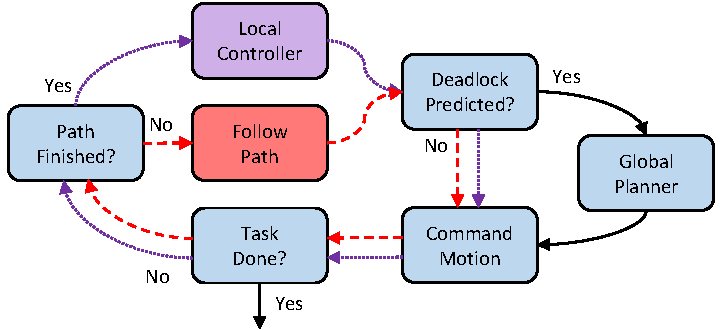
\includegraphics[width=\columnwidth]{FrameworkBlockDiagram}
    \caption{Block diagram showing the major components of our framework. On each cycle we use either the local controller (dotted purple arrows) or a planned path (dashed red arrows) to predict if the system will be deadlocked in the future, planning a new path is needed to avoid deadlock.}
    \label{fig:main_loop_diagram}
\end{figure}

Global planners are effective at finding paths through complex configuration spaces, but for highly underactuated systems such as deformable objects achieving a specific configuration is very difficult even with high-fidelity models; this means that we cannot rely on them to complete a task independent of a local controller. In order for the local controller to complete the task, the system must be in the correct basin of attraction. From this point of view it is not the planner's responsibility to complete a task but rather to move the system into the right basin for the local controller to finish the task. By explicitly separating planning from control we can use different representations of the deformable object for each component; this allows us to use a highly-simplified model of the deformable object for global planning to generate gross motion of the deformable object, while using an independent local approximation for the controller. The key question then is when should we use global planning versus local control?

Our framework can be broken down into three major components: (1) A global motion planner to generate gross motion of the deformable object; (2) A local controller for refinement of the configuration of the deformable object; and (3) A novel deadlock prediction algorithm to determine when to use planning versus control. Fig.~\ref{fig:main_loop_diagram} shows how these components are connected, switching between a local controller loop and planned path execution loop as needed. In the following sections we describe each component in turn, starting with the local controller.


\subsection{Local Control}
\label{sec:local_control}

The role of the local controller is not to perform the whole task, but rather to refine the configuration of the deformable object locally. For our local controller we use a controller of the form introduced in \cite{Berenson2013} and \cite{McConachie2018}. These controllers locally minimize error $\errorfunction$ while avoiding robot collision and excessive stretching of the deformable object.

An outline of how these controllers function is shown in Alg.~\ref{alg:local_controller}; 
first, for every target point $\deformtarget_i \in \deformtarget$ we define a workspace navigation function pointing towards $\deformtarget_i$ using Dijkstra's algorithm. This gives us the shortest collision-free path between any point in the workspace and the target point, as well as the distance travelled along that path. These navigation functions are used to define the best direction to move the deformable object $\deformvelocity_e$ and the relative importance of each part of the motion $\pseudoinverseweight_e$ in order to locally reduce error as much as possible at each timestep (Lines 1 and 2). These error reduction terms are then combined with stretching avoidance terms $\deformvelocity_s, \pseudoinverseweight_s$ to define the desired manipulation direction and importance weights $\deformvelocity_d, \pseudoinverseweight_d$ at each timestep (Lines 3 and 4). We then find the best robot motion to achieve the desired deformable object motion, while preventing collision between the robot and obstacles (Line 5).

Given the current system state $(\robotconfig, \deformconfig)$ FindBestRobotMotion$(\robotconfig, \deformconfig, \deformvelocity_d, \pseudoinverseweight_d)$ is solving the following problem:
\begin{equation}
\begin{aligned}
    & \argmin_{\robotvelocity } 
        & & \| f(\robotconfig, \deformconfig, \robotvelocity) - \deformvelocity_d \|_{\pseudoinverseweight_d} \\
    &\text{subject to}
        & & \| \robotvelocity \| \leq \maxrobotvel \\
    &   & & \left(\robotconfig + \robotvelocity\right) \in \cfree_r \enspace .
\end{aligned}
\label{eqn:controller_minimization_problem}
\end{equation}
How Eq.~\eqref{eqn:controller_minimization_problem} is solved depends on the particular robot; details for each function in Alg.~\ref{alg:local_controller} are in Appendix~\ref{apx:local_control}.


\begin{algorithm}[t]
    \caption{LocalController$(\robotconfig, \deformconfig, \deformtarget, \relaxeddistancematrix, \maxstretchfactor, \stretchingcorrectionweightfactor)$}
    \begin{algorithmic}[1]
        \State $\correspondences \gets$ CalculateCorrespondences$(\deformconfig_t, \deformtarget)$
        \State $\deformvelocity_e, \pseudoinverseweight_e \gets$ FollowNavigationFunction$(\deformconfig_n, \correspondences)$
        \State $\deformvelocity_s, \pseudoinverseweight_s \gets$ StretchingCorrection$(\relaxeddistancematrix, \maxstretchfactor, \deformconfig)$
        \State $\deformvelocity_d, \pseudoinverseweight_d \gets$ CombineTerms$(\deformvelocity_e, \pseudoinverseweight_e, \deformvelocity_s, \pseudoinverseweight_s, \stretchingcorrectionweightfactor)$
        \State $\robotcommandvel \gets$ FindBestRobotMotion$(\robotconfig, \deformconfig, \deformvelocity_d, \pseudoinverseweight_d)$
    \end{algorithmic}
    \label{alg:local_controller}
\end{algorithm}


An important limitation of this approach is that the individual navigation functions are defined and applied independently of each other; this means that the navigation functions that are combined to define the direction to move the deformable object can cause the controller to move the end effectors on opposite sides of an obstacle, leading to poor local minima, i.e. becoming stuck. Figure~\ref{fig:overstretch_example} shows our motivating example of this type of situation. Other examples of this kind of situation are shown in Section \ref{sec:simulation_experiments}. In addition, while this local controller prevents collision between the robot and obstacles, it does not explicitly have any ability to \textit{go around} obstacles.

In order to address these limitations we introduce a novel deadlock prediction algorithm to detect when the system $(\robotconfig[t], \deformconfig_t)$ is in a state that will lead to deadlock (i.e. becoming stuck) if we continue to use the local controller.


\begin{figure}[t]
    \centering
    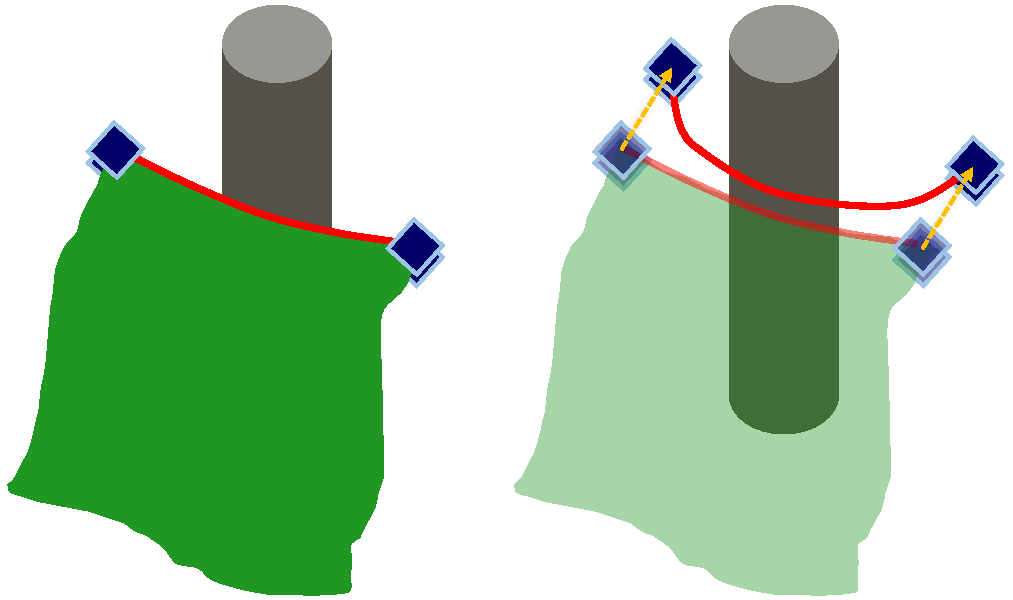
\includegraphics[width=\columnwidth]{OverstretchExample}
    \caption{Motivating example for deadlock prediction. The local controller moves the grippers on opposite sides of an obstacle, while the geodesic between the grippers (red line) cannot move past the pole, eventually leading to overstretch or tearing of the deformable object if the robot does not stop moving towards the goal.}
    \label{fig:overstretch_example}
\end{figure}



\subsection{Predicting Deadlock}
\label{sec:predicting_deadlock}



Predicting deadlock is important for two reasons; first we do not want to waste time executing motions that will not achieve the task. Second, we want to avoid the computational expense of planning our way out of a cul-de-sac after reaching a stuck state. By predicting deadlock before it happens we address both of these concerns. The key idea is to detect situations similar to Figure~\ref{fig:overstretch_example} where the local controller will wrap the deformable object around an obstacle without completing the task. We also need to detect situations where no progress can be made due to an obstacle directly in the path of the desired motion of the robot.



Let $\truemotion(\robotconfig, \deformconfig, \robotcommandvel) = \robotactualvel$ be the true motion of the robot when $\robotcommandvel$ is executed for unit time; in this section we will be predicting the future state of the system, thus it is not sufficient to consider only $\robotcommandvel$, we must also consider $\robotactualvel$.  Modelling inaccuracies as well as the deformable object being in contact can lead to meaningful differences between $\robotcommandvel$ and $\robotactualvel$. Specifically, when a deformable object is in contact with the environment, tracking $\robotcommandvel$ perfectly may lead to a constraint violation (i.e. overstretch or tearing of the deformable object).

We consider a controller to be deadlocked if the commanded motion produces (nearly) no actual motion, and the task termination condition is not met:
\begin{equation}
    \begin{split}
        \| \robotactualvel[t] \|               &\approx 0 \\
        \terminationcondition(\deformconfig_t) &= \texttt{false}.
        \label{eqn:stuck}
    \end{split}
\end{equation}
In general we cannot predict if the system will get stuck in the limit; to do so would require a very accurate simulation of the deformable object. Instead we predict if the system will get stuck within a prediction horizon $\predictionhorizon$ timesteps. We divide our deadlock prediction algorithm into three parts and discuss each in turn: 1) estimating gross motion; 2) predicting overstretch; and 3) progress detection.



\subsubsection{Estimating Gross Motion:}

The idea central to our prediction (Alg.~\ref{alg:predict_deadlock}) is that while we may not be able to determine precisely how a given controller will steer the system, we can capture the gross motion of the system and estimate if the controller will be deadlocked. We split the prediction into two parts; first we assume that controller $\controller$ is able to manipulate the deformable object with a reasonable degree of accuracy within a local neighborhood of the current state. This allows us to approximate the motion of the deformable object by following the task-defined navigation functions for each $\deformconfig_i \in \deformconfig$. Examples of this approximation are shown in Figure~\ref{fig:gross_deformable_motion}.

Next we use a simplified version of LocalController() which omits the stretching avoidance terms (Alg.~\ref{alg:local_controller} lines 3 and 4) to predict the commands sent to the robot. These terms are omitted as they can be sensitive to the exact configuration of the deformable object, which is not considered in this approximation. If we are executing a path then we can use the planned path directly to predict overstretch.



\begin{algorithm}[t]
\caption{PredictDeadlock$($\parbox[t]{1.5in}{$\errorfunction, \robotconfig[t], \deformconfig_t, \band_t, \deformtarget,$\\$\maxbandlength, \predictionhorizon,\textrm{Path})$}}
\begin{algorithmic}[1]
    \State ConfigHistory $\gets [\textrm{ConfigHistory}, q_t]$
    \State ErrorHistory $\gets [\textrm{ErrorHistory}, \errorfunction(\deformconfig_t)]$
    \State BandPredictions $\gets []$
    \State $\correspondences \gets$ CalculateCorrespondences$(\deformconfig_t, \deformtarget)$
    \For{$n = t, \dots, t + \predictionhorizon - 1$}
        \If {Path $\neq \emptyset$}
            \State $\deformvelocity_e, \pseudoinverseweight_e \gets$ FollowNavigationFunction$(\deformconfig_n, \correspondences)$
            \State $\deformconfig_{n + 1} \gets \deformconfig_n + \deformvelocity_e$
            \State $\robotcommandvel[n] \gets$ FindBestRobotMotion$($\parbox[t]{0.8in}{$\robotconfig[n], \deformconfig_{n},$ \\ $\deformvelocity_e, \pseudoinverseweight_e)$}
            \State $\robotconfig[n + 1] \gets \robotconfig[n] + \robotcommandvel[n]$
        \Else
            \State $\robotconfig[n + 1] \gets \robotconfig[n] + $ FollowPath(Path)
        \EndIf
        \State $\band_{n + 1} \gets$ ForwardPropagateBand$(\band_n, \robotconfig[n + 1])$
        \State BandPredictions $\gets [\textrm{BandPredictions}, \band_{n + 1}]$
    \EndFor
    \If {PredictOverstretch$(\textrm{BandPredictions},\ \maxbandlength)$ \textbf{or} \\NoProgress$($ConfigHistory, ErrorHistory$)$}
        \State \Return \texttt{true}
    \Else
        \State \Return \texttt{false}
    \EndIf
\end{algorithmic}
\label{alg:predict_deadlock}
\end{algorithm}


\begin{algorithm}[t]
\caption{ForwardPropagateBand$(\band, \robotconfig)$}
\begin{algorithmic}[1]
    \State $(p_0, p_1) \gets$ ForwardKinematics$(\robotconfig)$
    \State $\band \gets$ $[p_0, \band, p_1]$
    \State $\band \gets$ InterpolateBandPoints$(\band)$
    \State $\band \gets$ RemoveExtraBandPoints$(\band)$
    \State $\band \gets$ PullTight$(\band)$
    \State \Return $\band$
\end{algorithmic}
\label{alg:band_propogation}
\end{algorithm}





\subsubsection{Predicting Overstretch:}
\label{sec:overstretch}


Next we introduce the notion of a \textit{virtual elastic band} between the robot's end-effectors. This elastic band represents the shortest path through the deformable object between the end-effectors. The band approximates the constraint imposed by the deformable object on the motion of the robot; if the end-effectors move too far apart, then the elastic band will be too long, and thus the deformable object is stretched beyond a task-specified maximum stretching factor $\maxstretchfactor$. Similarly, if the elastic band gets caught on an obstacle and becomes too long, then the deformable object is also overstretched. By considering only the geodesic between the end-effectors, we are assuming that the rest of deformable object will comply to the environment, and does not need to be considered when predicting overstretch. The elastic band representation allows us to use a fast prediction method, but does not account for the part of the material that is slack. We discuss this trade-off further in Section \ref{sec:discussion}. This virtual elastic band is based on Quinlan's path deformation algorithm~\cite{Quinlan1994} and is used both in deadlock prediction as well as global planning (Sec.~\ref{sec:planning_goal} and Sec.~\ref{sec:global_planning})


Denote the configuration of an elastic band at time $t$ as a sequence of $\numbandpoints$ points $\band_t \subset \reals^3$. The number of points used to represent an elastic band can change over time, but for any given environment and deformable object there is an upper limit $\maxbandpoints$ on the number of points used. Define $\textrm{Path}(\band)$ to be the straight line interpolation of all points in $\band$. Define the length of a band to be the length of this straight line interpolation. At each timestep the elastic band is initialized with the shortest path between the end effectors through the deformable object, and then ``pulled'' tight using the internal contraction force described in ~\cite{Quinlan1994} \textsection5, and a hard constraint for collision avoidance. The endpoints of the band track the predicted translation of the end effectors (Alg.~\ref{alg:band_propogation}). This band represents the constraint that must be satisfied for the object not to tear. By considering only this constraint on the object in prediction, we are implicitly relying on the object to comply to contact as it is moved by the robot. We discuss the limitations of this assumption in the discussion (Sec.~\ref{sec:discussion}).



Let $\bandlength_{t+n}$ be the length of the path defined by the virtual elastic band $\band_{t+n}$ at timestep $n$ in the future, and $\maxbandlength$ be the longest allowable band length. To use this length sequence to predict if the controller will overstretch the deformable object, we perform three filtering steps: an annealing low-pass filter, a filter to eliminate cases where the band is in freespace, and the detector itself which predicts overstretch. We use a low-pass annealing filter with annealing constant $\bandlengthannealing \in [0, 1)$ to mitigate the effect of numerical and approximation errors which could otherwise lead to unnecessary planning:
\begin{equation}
    \begin{split}
        \tilde \bandlength_{t + 1} &= \bandlength_{t + 1} \\
        \tilde \bandlength_{t + n} &= \bandlengthannealing \tilde \bandlength_{t + n - 1} + (1 - \bandlengthannealing) \bandlength_{t + n} \enspace ,  n = 2, \dots, \predictionhorizon \enspace .
    \end{split}
\end{equation}
Second, we discard from consideration any bands which are not in contact with an obstacle; we can eliminate these cases because our local controller includes an overstretch avoidance term which will prevent overstretch in this case in general. Last we compare the filtered length of any remaining band predictions to $\maxbandlength$; if after filtering, there is an estimated band length $\tilde \bandlength$ that is larger than $\maxbandlength$ then we predict that the local controller will be stuck. An example of this type of detection is shown in Figure~\ref{fig:overstretch_predicted}, where the local controller will wrap the cloth around the pole, eventually becoming deadlocked in the process.




\begin{figure}
    \centering
    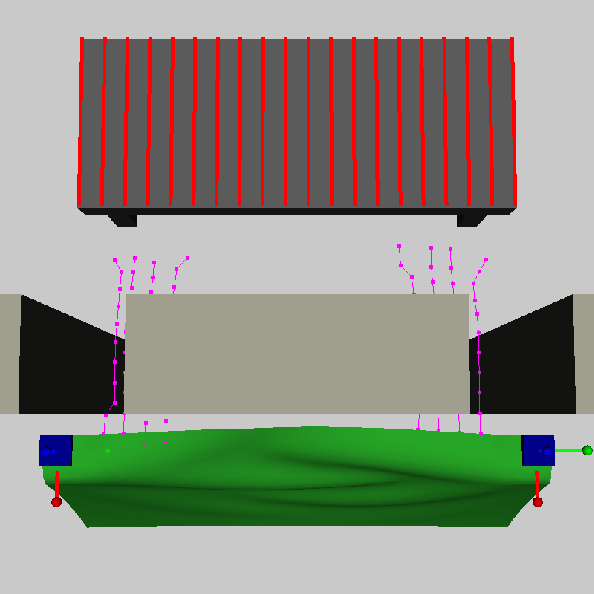
\includegraphics[width=\columnwidth]{GrossDeformableMotion}
    \caption{Example of estimating the gross motion of the deformable object for a prediction horizon $\predictionhorizon = 10$. The magenta lines start from the points of the deformable object that are closest to the target points (according to the navigation function). These lines show the paths those points would follow to reach the target when following the navigation function.}
    \label{fig:gross_deformable_motion}
\end{figure}

\begin{figure}
    \centering
    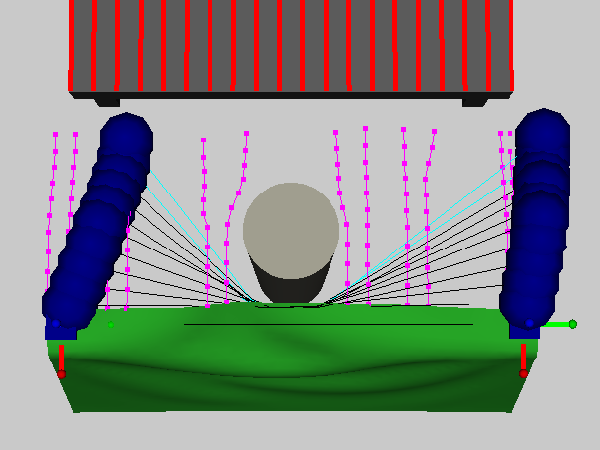
\includegraphics[width=\columnwidth]{OverstretchPredicted}
    \caption{Estimated gross motion of the deformable object (magenta lines) and end effectors (blue spheres). The virtual elastic band (black lines) is forward propagated by tracking the end effector positions, changing to cyan lines when overstretch is predicted.}
    \label{fig:overstretch_predicted}
\end{figure}







\subsubsection{Progress Detection:}

Last, we track the progress of the robot and task error to estimate if the controller $\controller$ is making progress towards the task goal. This is designed to detect cases when the robot is trapped against an obstacle. Naively we could look for instances when $\robotactualvel = 0$ however due to sensor noise, actuation error, and using discrete math in a computer, we need to use a threshold instead. At the same time we want to avoid false positives, where the robot is moving slowly but task error is decreasing. To address these concerns we record the configuration of the robot (stored in ConfigHistory) and the task error (stored in ErrorrHistory) every time we check for deadlock, and introduce three parameters to control what it means to be making progress: history window $\historywindow$, error improvement threshold $\errorprogressthreshold$, and configuration distance threshold $\motionprogressthreshold$. If over the last $\historywindow$ timesteps, the improvement in error is less than $\errorprogressthreshold$, and the robot has moved less than $\motionprogressthreshold$, then we predict that the controller will not be able to reach the goal from the current state and trigger global planning.



\subsection{Setting the Global Planning Goal}
\label{sec:planning_goal}


In order to enable efficient planning, we need to approximate the configuration of the deformable object in a way that captures the gross motion of the deformable object without being prohibitively expensive to use. We use the same approach from Sec.~\ref{sec:overstretch}, but the interpretation in this use is slightly different; the virtual elastic band is a proxy for the leading edge of the deformable object. In this way we can plan to move the deformable object to a different part of the workspace without needing to simulate the entire deformable object, instead the deformable object conforms to the environment naturally.



In order to make progress towards achieving the task, we want to set the goal for the global planner to be a configuration that we have not explored with the local controller. We do so in two parts; we find the set of all target points $\deformtarget_U$ which are contributing to task error, split these points into two clusters, and use the cluster centers to define the goal region of the end effectors, $\eepositiongoal$; any end-effector position within a task-specified distance $\goalreachradius$ is considered to have reached the end-effector goal (Alg.~\ref{alg:call_global_planner} lines 1-3). Second, we set the goal configuration of the virtual elastic band to be any configuration that is not similar to a \textit{blacklist} of virtual elastic bands. This blacklist is the set of all band configurations from which we predicted that the local controller would be deadlocked in the future (Sec.~\ref{sec:predicting_deadlock}).


To define similarity we use Jaillet and Sim\'{e}on's \textit{visibility deformation} definition to compare two virtual elastic bands (\cite{Jaillet2008}). Intuitively two virtual elastic bands are similar if you can sweep a straight line connecting the two bands from the start points to the end points of the two bands without intersecting an obstacle. Unlike the original use, we do not constrain the start and end points of each path to match, but the algorithm is identical. We use this as a heuristic to find states that are dissimilar from states where we have already predicted that the local controller would be deadlocked. Let VisCheck$(\band,\textrm{Blacklist}) \rightarrow \{0, 1\}$ denote this visibility deformation check, returning $1$ if $\band$ is similar to a band in the blacklist and $0$ otherwise. Then
\begin{equation}
    \bandgoal = \{\band \mid \text{VisCheck}(\band, \textrm{Blacklist}) = 0\}
    \label{eqn:bandgoal}
\end{equation}
is the set of all virtual elastic bands that are dissimilar to the Blacklist.

Combined, $\eepositiongoal, \goalreachradius$, and $\bandgoal$ define what it means for the planner to have found a path to the goal (Alg.~\ref{alg:goal_check}); the end-effectors must be in the right region, and the virtual elastic band must be dissimilar to any band in the Blacklist.%\todo{$\rrtnodeset$ is not yet defined}



\begin{algorithm}[t]
\caption{PlanPath$($\parbox[t]{1.8in}{$\robotconfig[t], \deformconfig_t, \band_t, \deformtarget, \goalreachradius,$\\
                                      $\maxbandlength, \bestneardist, \textrm{Blacklist})$}}
\begin{algorithmic}[1]
    \State $\deformtarget_U \gets$ UncoveredTargetPoints$(\deformconfig_t, \deformtarget)$
    \State $\eepositiongoal \gets$ ClusterCenters$(\deformtarget_U)$
    \State $\eepositiongoal \gets$ ProjectOutOfCollision$(\eepositiongoal)$
    \State $\bandgoal \gets \{\band \mid \text{VisCheck}(\band, \text{Blacklist}) = 0\}$
    \State Path $\gets$ RRT-EB$(\robotconfig[t], \band_t, \eepositiongoal, \goalreachradius, \bandgoal, \maxbandlength, \bestneardist)$
    \If {Path $\neq$ Failure}
        \State \Return ShortcutSmooth(Path)
    \Else
        \State \Return Failure
    \EndIf
\end{algorithmic}
\label{alg:call_global_planner}
\end{algorithm}


\begin{algorithm}[t]
\caption{GoalCheck$(\rrtnodeset, \eepositiongoal, \goalreachradius, \bandgoal)$}
\begin{algorithmic}[1]
    \For {$\config_f = (\robotconfig, \band) \in \rrtnodeset$}
        \State $(p_0, p_1) \gets$ ForwardKinematics$(\robotconfig)$
        \If {$\|p_0 - \eepositiongoal[0] \| \leq \goalreachradius$ \textbf{and} \\
             $\|p_1 - \eepositiongoal[1] \| \leq \goalreachradius$ \textbf{and} $\band \in \bandgoal$}
            \State \Return 1
        \EndIf
    \EndFor
    \State \Return 0
\end{algorithmic}
\label{alg:goal_check}
\end{algorithm}




The combination of local control, deadlock prediction, and global planning are shown in the MainLoop function (Alg.~\ref{alg:mainloop}). Because the virtual elastic band is an approximation we need to predict deadlock while executing the planned path. We use the same prediction method for path execution as for the local controller. To set the maximum band length $\maxbandlength$ used by the global planner and the deadlock prediction algorithms, we calculate the geodesic distance between the grippers through the deformable object in its ``laid-flat'' state and scale it by the task specified maximum stretching factor $\maxstretchfactor$.




